% 原书 p.25–p.29（PDF p.33–p.37）
% >>> p033
\section{哈密顿力学（Hamiltonian Mechanics）}

\begin{keytakeaways}
\begin{itemize}
  \item 物理图像：同一个力学系统在余切丛 $T^*\R^2$ 上由哈密顿函数 $H(q,p)$ 与哈密顿流描述，
        相空间中的轨迹是哈密顿向量场 $X_H$ 的积分曲线。
  \item 数学工具：标准辛形式 $\omega_{\mathrm{can}}=\sum_i\dd p_i\wedge\dd q_i$、
        内乘 $\iota_{X_H}$、哈密顿向量场与梯度向量场的关系、Legendre 变换
        $\mathcal{L}(f)(p)=px(p)-f(x(p))$。
  \item 几何观点：拉格朗日量关于速度的严格凸性保证 $v\mapsto p=\partial_vL$ 可逆，
        从而把切丛上的二阶 Euler--Lagrange 方程化为余切丛上的一阶哈密顿方程 (2.6)；
        $X_H$ 是 $H$ 的「辛梯度」，与欧氏梯度 $\nabla H$ 逐点正交。
  \item 本节结论：命题 2.2.1——Euler--Lagrange 方程与哈密顿方程在 Legendre 变换下等价；
        对幂函数 $Cx^\alpha$ 的计算表明，Legendre 变换把幂次 $\alpha$ 变为其 Hölder 共轭
        $\alpha/(\alpha-1)$。
\end{itemize}
\end{keytakeaways}

本节我们将说明，如何通过一个简单却深刻的变换，把 (2.2) 中的 Euler--Lagrange 方程与哈密顿系统联系起来。

回顾：在 $T^*\R^2$ 上存在辛结构 $\omega_{\mathrm{can}}$（见例 1.2.2）。给定 $T^*\R^2$ 上的哈密顿函数 $H$，由定义 1.7.1，哈密顿向量场 $X_H$ 由下式给出：
\begin{equation}
  \dd H=-\iota_{X_H}\omega_{\mathrm{can}}
  \qquad\text{其中}\qquad
  \omega_{\mathrm{can}}=\sum_{i=1}^2\dd p_i\wedge\dd q_i .
  \tag{2.4}
\end{equation}
% [Tutor Note: 易错预警——本书采用 $\dd H=-\iota_{X_H}\omega$ 的符号约定（与定义 1.7.1 一致）；不少教材（如 McDuff--Salamon）写作 $\iota_{X_H}\omega=\dd H$，两者相差一个整体符号，会连带改变哈密顿方程的符号。全书统一按本书约定。另外 $\omega_{\mathrm{can}}=\sum_i\dd p_i\wedge\dd q_i$ 与 $\sum_i\dd q_i\wedge\dd p_i$ 也只差符号，须与 (2.5)、(2.6) 中的下标位置对照核对。]
% >>> p034
设 $X_H=A\dfrac{\partial}{\partial q_1}+B\dfrac{\partial}{\partial q_2}+C\dfrac{\partial}{\partial p_1}+D\dfrac{\partial}{\partial p_2}$（系数为 $A,B,C,D$），我们可如下解方程 (2.4)。在坐标 $(q,p)$ 下，(2.4) 等价于
\[
  \dd H=\sum_{i=1}^2\frac{\partial H}{\partial q_i}\dd q_i
  +\sum_{i=1}^2\frac{\partial H}{\partial p_i}\dd p_i,
\]
以及
\[
  -\iota_{X_H}\omega_{\mathrm{can}}
  =-\Big(\sum_{i=1}^2\dd p_i\wedge\dd q_i\Big)(X_H,\cdot)
  =-C\dd q_1+A\dd p_1-D\dd q_2+B\dd p_2 .
\]
比较系数，得
\begin{equation}
  X_H=\frac{\partial H}{\partial p_1}\frac{\partial}{\partial q_1}
  +\frac{\partial H}{\partial p_2}\frac{\partial}{\partial q_2}
  -\frac{\partial H}{\partial q_1}\frac{\partial}{\partial p_1}
  -\frac{\partial H}{\partial q_2}\frac{\partial}{\partial p_2}.
  \tag{2.5}
\end{equation}
令 $\eta=\{(q(t),p(t))\}_{t\in[0,1]}$ 表示 $X_H$ 的积分曲线，即 $\dot\eta(t)=X_H(\eta(t))$。于是得到一阶微分方程组，称为\textbf{哈密顿方程}：
\begin{equation}
  \begin{cases}
    \dot q_i(t)=\dfrac{\partial H}{\partial p_i}(q(t),p(t))\\[2mm]
    \dot p_i(t)=-\dfrac{\partial H}{\partial q_i}(q(t),p(t))
  \end{cases}
  \qquad\text{对 } i=1,2 .
  \tag{2.6}
\end{equation}
注意这里总共有四个微分方程（而在同样的设定下，(2.2) 只有两个微分方程）。
% [Tutor Note: (2.6) 中两个方程共用同一个自由指标 $i=1,2$，故实际写开为四条一阶方程；变量为 $(q_1,q_2,p_1,p_2)$。这也解释了为何哈密顿形式把二阶方程降阶：相空间维数加倍，换得一阶方程组。]

\begin{wrem}{2.2.1}
回顾 $H$ 的梯度有如下表达式
\[
  \nabla H=\frac{\partial H}{\partial q_1}\frac{\partial}{\partial q_1}
  +\frac{\partial H}{\partial q_2}\frac{\partial}{\partial q_2}
  +\frac{\partial H}{\partial p_1}\frac{\partial}{\partial p_1}
  +\frac{\partial H}{\partial p_2}\frac{\partial}{\partial p_2}.
\]
与 (2.5) 中 $H$ 的哈密顿向量场相比较，可知 $X_H\perp\nabla H$。梯度向量场 $\nabla H$（及其生成的梯度流）有清晰的几何意义，而由哈密顿向量场 $X_H$ 给出的正交方向，多少以一种「水平」的方式，生成一个更为神秘的流——哈密顿流（见定义 1.7.1）。
% [Tutor Note: 这里的「$X_H\perp\nabla H$」是相对于坐标 $(q,p)$ 所诱导的欧氏度量而言：直接计算得 $\langle X_H,\nabla H\rangle=\sum_i(\partial_{p_i}H)(\partial_{q_i}H)-\sum_i(\partial_{q_i}H)(\partial_{p_i}H)=0$。它并非辛结构的内蕴性质；在一般辛流形上「正交」须先选定相容的近复结构 $J$ 与度量 $g(\cdot,\cdot)=\omega(\cdot,J\cdot)$ 才有意义。]
\end{wrem}

\begin{wprop}{2.2.1}
(2.2) 中定义的 Euler--Lagrange 方程与 (2.6) 中的哈密顿方程等价。
\end{wprop}

上面命题 2.2.1 的粗略陈述可能引起误解，因为这两个方程组甚至不是定义在同一个空间上（一个在 $T\R^2$ 上，另一个在 $T^*\R^2$ 上）。因此，正如预期，$T\R^2$ 与 $T^*\R^2$ 之间应存在某种变换，称为 \textbf{Legendre 变换}，它由 A. M. Legendre 于 1787 年引入 [146]。

下面用一个玩具式的情形来演示 Legendre 变换。对任意光滑函数 $f$，其图像既可由点 $(x,f(x))$ 给出，也可由切线 $Y=f'(x)X-c(x)$ 给出，其中变量为 $Y$ 与 $X$，而 $c(x)$ 是负的 $y$ 截距。
% >>> p035
在切线方程中取 $X=x$，便得到如下同义反复的关系式
\begin{equation}
  f(x)=f'(x)x-c(x).
  \tag{2.7}
\end{equation}
见图 2.2：若给定的 $f$ 严格凸，则其导数 $f'(x)$ 是（严格）单调的，于是 $f'(x)$ 与 $x$ 之间存在一一对应。这促使我们引入新变量 $p:=f'(x)$，并把对应的表达式 $x=x(p)$ 看作 $p$ 的函数。注意 $x$ 是良定义的。回到 (2.7)，它可重写为
\[
  f(x(p))=px(p)-c(x(p))
  \qquad\text{或等价地}\qquad
  c(x(p))=px(p)-f(x(p)).
\]
换言之，我们把直线的「点–值」描述替换为另一种「斜率–截距」描述。

\begin{figure}[htbp]
  \centering
  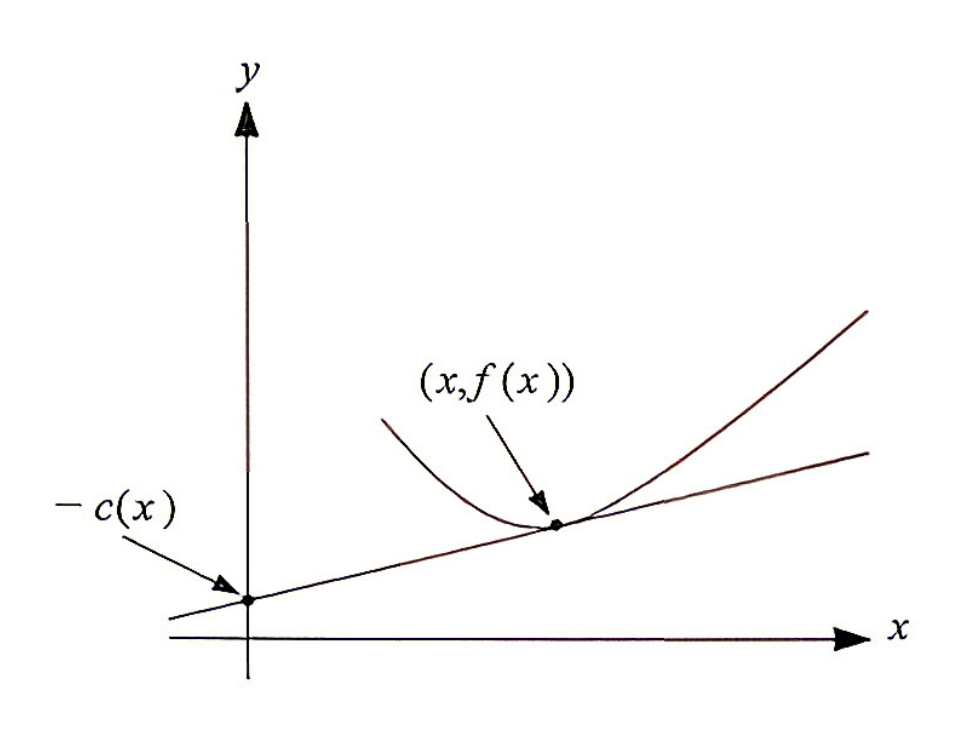
\includegraphics[width=0.62\linewidth]{figures/fig_p035_1.png}
  \caption*{图 2.2\quad $c(x)$ 与 $f(x)$ 的对应关系（原书 p.27, Figure 2.2；PDF p.35）}
\end{figure}

\begin{wdefn}{2.2.1}
对 $\R$ 上的严格凸函数 $f=f(x)$，我们借助斜率 $p$ 定义新函数 $\mathcal{L}(f)$：
\[
  \mathcal{L}(f)(p):=px(p)-f(x(p)),
\]
并称 $\mathcal{L}(f)$ 为 $f$ 的 \textbf{Legendre 变换}（Legendre transform）。
\end{wdefn}
% [Tutor Note: 术语与记号——原文用花体 $\mathcal{L}$ 表示 Legendre 变换算子，与拉格朗日量 $L$ 区分；请勿混淆。严格凸性保证 $f'$ 可逆，从而 $\mathcal{L}(f)$ 是良定义的；在凸分析中这就是 Legendre--Fenchel 变换。Legendre 变换是对合（involutive）的：$\mathcal{L}(\mathcal{L}(f))=f$（在严格凸、适当正则的假设下），这可作为习题验证。]

\begin{wrem}{2.2.2}
定义 2.2.1 中所定义的变换容易推广到高维情形。
\end{wrem}

下面是最基本的例子。

\begin{wexam}{2.2.1}
考虑 $f(x)=\dfrac{x^2}{2}$。则 $p=f'(x)=x$，即 $x=x(p)=p$。由定义 2.2.1，得
\[
  \mathcal{L}(f)(p)=p\cdot p-f(p)=p^2-\frac{p^2}{2}=\frac{p^2}{2}.
\]
% >>> p036
一般地，考虑 $f(x)=Cx^\alpha$，其中 $\alpha>1$。则 $p=f'(x)=\alpha Cx^{\alpha-1}$，其中 $\alpha-1>0$。于是 $x=x(p)=\left(\dfrac{p}{\alpha C}\right)^{\frac{1}{\alpha-1}}$。由定义 2.2.1，得
\begin{align*}
  \mathcal{L}(f)(p)
  &=p\left(\frac{p}{\alpha C}\right)^{\frac{1}{\alpha-1}}
    -C\left(\frac{p}{\alpha C}\right)^{\frac{\alpha}{\alpha-1}}\\
  &=\left(\left(\frac{1}{\alpha C}\right)^{\frac{1}{\alpha-1}}
    -C\left(\frac{1}{\alpha C}\right)^{\frac{\alpha}{\alpha-1}}\right)
    p^{\frac{\alpha}{\alpha-1}}.
\end{align*}
注意 Legendre 变换把 $f(x)$ 中原有的幂次 $\alpha$ 变为 $\mathcal{L}(f)$ 中的 Hölder 共轭 $\dfrac{\alpha}{\alpha-1}$。\hfill$//$
\end{wexam}

下面再看一个与例 2.1.1 中所考虑的拉格朗日量有关的具体例子。

\begin{wexam}{2.2.2}
回忆拉格朗日量 $L$ 由
\[
  L(q,v)=\frac12m|v|^2-V(q)
\]
定义，其中 $V(q)$ 表示势能。则 $p=\partial_vL(q,v)=mv$，这在物理学中称为经典动量。于是 $v=v(p)=\dfrac{p}{m}$。由定义 2.2.1，得
\[
  \mathcal{L}(L(q,\cdot))(p)=p\cdot\frac{p}{m}
  -\frac12m\left(\frac{p}{m}\right)^2+V(q)
  =\frac{p^2}{2m}+V(q).
\]
注意最后的结果 $\dfrac{p^2}{2m}+V(q)$ 恰是该系统的总能量。\hfill$//$
% [Tutor Note: 这里的计算要点是：$H=\mathcal{L}(L(q,\cdot))(p)=pv-L(q,v)$ 在 $p=\partial_vL$ 处取值，且 $\mathcal{L}(L(q,\cdot))$ 对每个固定 $q$ 只对速度变量作变换。$p^2/(2m)$ 是动能、$V(q)$ 是势能，二者之和即总能量——这正是 §2.1 所述「拉格朗日量 $=$ 动能 $-$ 势能」的直接对偶。]
\end{wexam}

\begin{wexer}{2.2.1}
算出例 2.1.2 中 $L$ 的 Legendre 变换。更确切地说，对每一点 $q=(q_1,q_2)\in M$，计算 $\mathcal{L}(L(q,\cdot))$。
\end{wexer}

现在可以给出命题 2.2.1 的证明了，其关键是引入新变量——动量 $p=\partial_vL(q,v)$。

\begin{wproof}[命题 2.2.1 的证明]
设 $L=L(q,v):T\R^2\to\R$ 是定义 2.1.1 与事实 2.1.1 中所述的那种严格凸函数，考虑其 Legendre 变换 $H:=\mathcal{L}(L):T^*\R^2\to\R$。注意 $H=H(q,p)$，其中 $p=\partial_vL(q,v)$（更确切地说，$p_i=\partial_{v_i}L(q_1,q_2,v_1,v_2)$，$i=1,2$）。由定义 2.2.1，$H(q,p)=pv(p)-L(q,v(p))$。于是对 $i=1,2$，有
\[
  \frac{\partial H}{\partial q_i}=-\frac{\partial L}{\partial q_i}
  =-\frac{\dd}{\dd t}\frac{\partial L}{\partial v_i}=-\dot p,
\]
其中第二个等号来自 (2.2)。类似地，有
\[
  \frac{\partial H}{\partial p_i}
  =v_i(p)+\left(p_iv_i'(p)-\frac{\partial L}{\partial v_i}v_i'(p)\right)=v_i(p)=\dot q .
\]
% [Tutor Note: 原文疑误——命题开头的定义域应写作 $L=L(q,v):T\R^2\to\R$（与定义 2.1.1、事实 2.1.1 一致），其 Legendre 变换才落在 $T^*\R^2$ 上；原文误写为 $T^*\R^2$。译文保留原文写法，详见 review_ch02.md。另注：上式中的 $v_i'(p)$ 意为 $\partial v_i/\partial p_i$，此处 $i$ 不求和；先证 $\partial H/\partial q_i=-\partial L/\partial q_i$ 时须注意求偏导时 $p$ 固定、而 $v=v(p)$ 与 $q$ 无关。]
最后一个等号成立，是因为我们是在轨迹 $(\gamma(t),\gamma'(t))$ 上对所有涉及的函数取值。于是，若 $\gamma(t)=(q_1(t),q_2(t))$，则速度分量为 $v_i=\dot q_i$（$i=1,2$）。因此我们确认 (2.2) 蕴含 (2.6)。反过来的验证是类似的，留给有兴趣的读者。
\end{wproof}

% >>> p037
由命题 2.2.1 可知，描述一个力学系统有两种等价的方式，通常分别称为拉格朗日力学与哈密顿力学。两者各有其优点，并构成物理学中许多高级课题的基础（见 [96] 第 8 章）。

